% !TEX encoding = UTF-8
% !TEX TS-program = pdflatex
% !TEX root = ../tesi.tex

%**************************************************************
\chapter{Processi e metodologie}
\label{cap:processi-metodologie}
%**************************************************************

Durante il periodo di stage, ho avuto l'opportunità di entrare in contatto con i processi aziendali e diversi strumenti a supporto del mio lavoro, di seguito illustrati.

\section{Accertamento di Qualità}

Il processo di Accertamento di qualità provvede a garantire che il prodotto software sia conforme alle aspettative di qualità desiderate. Nello specifico, durante il mio periodo di stage, sono venuto a contatto con le seguenti pratiche di sviluppo.

\subsection{Pull Request}

\begin{figure}[H] 
  \centering 
  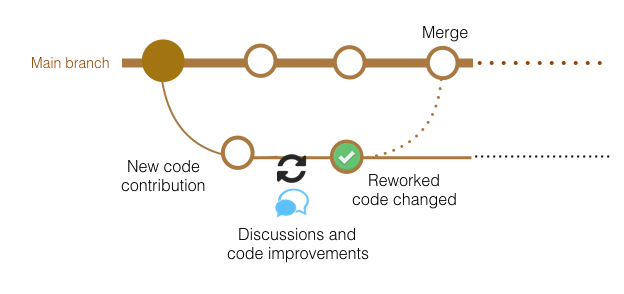
\includegraphics[width=0.75\columnwidth]{pull-request} 
  \caption{Flusso di una Pull Request}
\end{figure}

Una Pull Request è una proposta di modifica al repository effettuata su Github. Essa è obbligatoria per qualsiasi modifica e deve essere sempre realizzata tramite un git branch dedicato, avente un nome univoco e semantico rispetto alle modifiche proposte. \\

Lo scopo della Pull Request in WorkWave è favorire la discussione delle modifiche da parte del team e permetterne un'attenta ispezione prima di ritenerla valida. Tuttavia essa è anche un'opportunità di apprendimento sia per chi esegue la review che per chi la riceve, in quanto entrambi hanno modo di apprendere diversi approcci allo stesso problema. \\

Essa permette anche, nel lungo termine, di venire a conoscenza di problematiche nel processo di sviluppo e poterle migliorare. Ad esempio la continua segnalazione di norme di sintassi è un indice della necessità di introdurre uno strumento automatico per la formattazione del codice.

\section{Gestione della configurazione}

\subsection{Versionamento}

L'azienda WorkWave organizza il proprio codice sorgente all'interno di diverse repository Git raggruppate sotto l'organizzazione GitHub dell'azienda. \\

In particolare è stato creato un repository dedicato al versionamento della prima fase della libreria \textit{Stargate} assieme al Proof of Concept. Successivamente il codice sorgente della libreria è stato direttamente integrato nel repository dell'applicazione \textit{Route Manager}.

\subsection{Ambiente di verifica}

\begin{figure}[H] 
  \centering 
  
\includegraphics[width=0.5\columnwidth]{jenkins} 
  \caption{Jenkins}
\end{figure}

Il processo di verifica è il più automatizzato possibile tramite tools eseguiti automaticamente con Jenkins \url{https://jenkins.io/}. Lo stesso procedimento avviene ad ogni Pull Request proibendone l’accettazione se le verifiche non sono superate.

Inoltre sono presenti script automatici che permettono di rilasciare in ambiente di sviluppo, demo, testing e produzione attraverso l'interfaccia grafica dashboard di Jenkins.

\subsection{Ambiente di rilascio}

\begin{figure}[H] 
  \centering 
  
\includegraphics[width=0.5\columnwidth]{clodfront} 
  \caption{Amazon Cloudfront}
\end{figure}

Il rilascio automatico eseguito da Jenkins porta al caricamento dell'applicazione \textit{Route Manager} su Amazon Cloudfront \url{https://aws.amazon.com/it/cloudfront/}, un servizio di Content Delivery Network (CDN) che permette di distribuire l'applicazione con latenza minima nei diversi Paesi del mondo.

\section{Gestione di Progetto}

\subsection{Standup}

Il team si incontra quotidianamente per lo standup, un incontro informale senza durata prefissata, che permette ai vari membri di allinearsi reciprocamente sullo stato di avanzamento ed eventuali problematiche. In particolare, nel caso di WorkWave tale attività è indispensabile in quanto vi sono alcuni del team che lavorano in remoto o negli Stati Uniti. \\

Tutti i membri, non solo i programmatori, sono invitati a partecipare e ad esporre su cosa stiano lavorando e potenziali criticità, permettendo anche di trasmettere maggiore consapevolezza e conoscenza del progetto ai diversi partecipanti.

\subsection{Ticketing}

\begin{figure}[H] 
  \centering 
  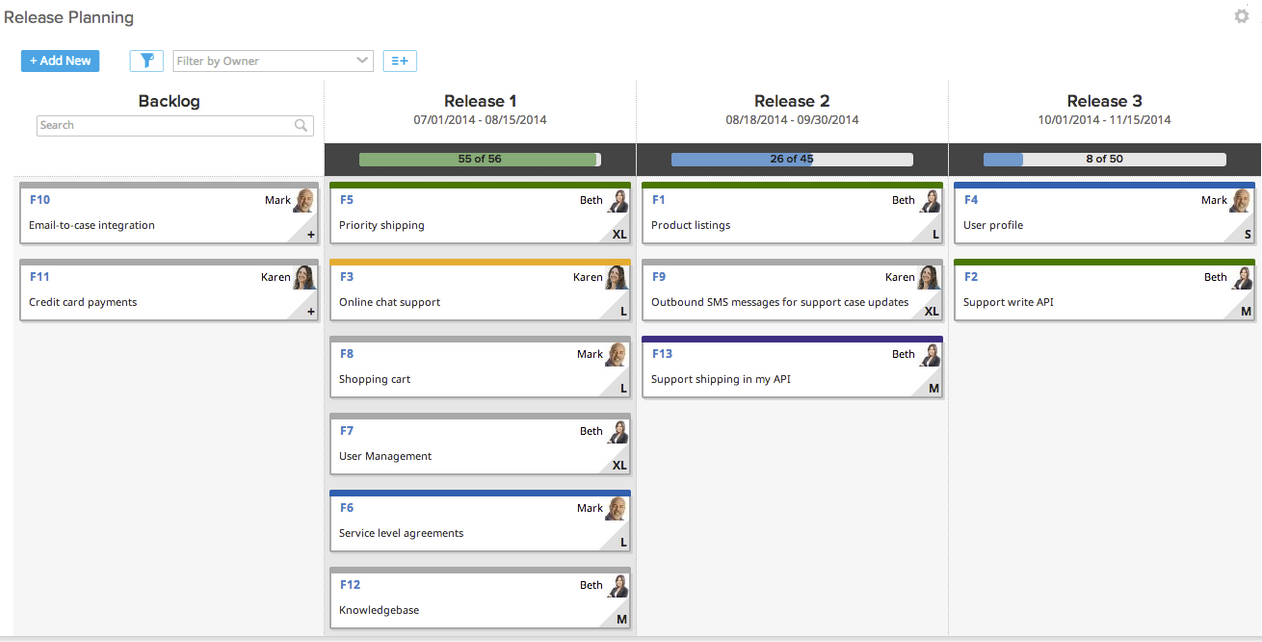
\includegraphics[width=1\columnwidth]{releaseplan_main} 
  \caption{CA Agile Central}
\end{figure}

L'azienda utilizza lo strumento CA Agile Central \footnote{ \url{https://www.ca.com/it/products/ca-agile-central.html}} per la gestione del ticketing, assegnando un ticket per ogni attività atomica. Ciò permette un'agevolazione nell'allineamento nel team sulle attività e gli obiettivi giorno per giorno. \\

Sono inoltre assegnate diverse priorità alle task al fine di garantire il completamento di quelle con maggior valore. Oltre a ciò è possibile avere un quadro complessivo del progresso, delle dipendenze e dell'allineamento della pianificazione durante ogni \gls{sprint}.
